% !TEX encoding = UTF-8 Unicode
% -*- coding: UTF-8; -*-

\documentclass[UTF8,hyperref]{pkuthss}

% 产生 originauth.tex 里的 \Square。
\usepackage{wasysym}
% 提供 verbatiminput 命令和 comment 环境。
\usepackage{verbatim}

% 设置页芯居中。
\geometry{centering}
% 设定行距。
\renewcommand{\baselinestretch}{1.5}

% 使引用标记成为上标。
\newcommand{\supercite}[1]{\textsuperscript{\cite{#1}}}
% 罗列环境中如果每个项目都只有一行左右,则会显得很松散,此时可采用这个命令。
\newcommand{\denselist}{\setlength{\itemsep}{0pt}}

\begin{document}
  %% 设定生成的 pdf 的文档信息。
  \hypersetup
  {
    pdfauthor={Hongjian Yang},
    pdftitle={大型触摸设备上的多点触控中文输入法实现},
    pdfsubject={北京大学本科生毕业论文},
    pdfkeywords={中文, 输入法, 多点触控, 多通道}
  }

  %% 各种文档信息。
  \renewcommand{\thesisname}{本科生毕业论文}
  % 题目一般不宜超过 20 个字。
  \title{大型触摸设备上的多点触控中文输入法实现}
  \etitle{Multi-touch Chinese Input Methods on Large Screen Device}
  \author{杨洪鉴}
  \eauthor{Hongjian\ Yang}
  \studentid{1100016617}
  \date{二〇一五年六月}
  \school{信息科学技术学院}
  \major{计算机}
  \emajor{Computer Science}
  \direction{人机交互}
  \mentor{王衡~教授}
  \ementor{Prof.\ Heng Wang}
  % 关键词应有 3~5 个。
  \keywords{中文, 输入法, 多点触控, 多通道}
  \ekeywords{Chinese, Input Method, Multitouch, Multichannel}

  %% 以下为正文之前的部分,页码为小写罗马数字。
  \frontmatter\pagenumbering{roman}

  % 自动生成标题页。
  \maketitle
  % 版权声明。
  % \cleardoublepage
\chapter*{\textbf{版权声明}}
{
	\zihao{3}
\begin{comment}
	任何收存和保管本论文各种版本的单位和个人,
	未经本论文作者同意,不得将本论文转借他人,
	亦不得随意复制、抄录、拍照或以任何方式传播。
	否则一旦引起有碍作者著作权之问题,将可能承担法律责任。
\end{comment}
	版权所有~\copyright~2008--2009 solvethis
	\par
	版权所有~\copyright~2010 Casper Ti. Vector
	\vspace{0.75em}\par
	本文档可在~GNU~自由文档许可证(GFDL)\footnote%
	{\ \url{http://www.fsf.org/licensing/licenses/fdl.html}}%
	的第~1.3~版(或之后任意版本)或~GNU~通用公共许可证(GPL)\footnote%
	{\ \url{http://www.fsf.org/licensing/licenses/gpl.html}}%
	的第~3~版(或之后任意版本)所规定的条款下自由地复制、修改和发布。
	
	以上所述两个许可证应该在本文档所在目录的~\verb|license/|~%
	\linebreak[1]子目录下,
	文件名分别为~\verb|fdl-1.3.txt|~和~\verb|gpl-3.0.txt|。
	如果没有,你可以到上面提到的网址查看许可证内容。
	如果还不行,请写信给下面的地址以获得邮寄的许可证:
\begin{verbatim}
    The Free Software Foundation, Inc.,
    675 Mass Ave, Cambridge, MA02139, USA 
\end{verbatim}
	\par
}


  % 中英文摘要。
  % !TEX encoding = UTF-8 Unicode
% -*- coding: UTF-8; -*-

% 摘要要求在 3000 字以内。

\cleardoublepage
\begin{cabstract}

  本文详细介绍了两种在触摸设备上的新型中文拼音输入方法。两种输入方法分别面向对拼音输入生疏和熟悉的两种不同的用户群,综合利用了触摸设备所提供的多点触摸功能,采用多通道输入的方式,意在为不同的用户群体提供更加便捷易用的交互手段。同时,本文对这两种新型输入法与多种传统拼音输入法进行了比较,包括了不同设备上的,拥有不同键盘布局的输入法,并分析了该输入法在触摸设备上的优势。最后,本文讨论了该输入法现阶段的不足已经的其后续拓展的方向。

\end{cabstract}

\cleardoublepage
\begin{eabstract}

  We present two kinds of Chinese Input Methods in multitouch device. These two methods are made respectively for people who familiar of unfamiliar with Pinyin input, taking the advantages of interactions provided by multitouch device and using multichannel techniques. We intend to provide more convenient and easier access to Chinese input for various users. Meanwhile, We compare our input methods to those already existed ones, including those on different devices and those have different layout. And we point out the advantages of ours. Finally, we discussed the disadvantages of our input methods for now and the possibilities of their future developments.

\end{eabstract}


  % 使 \pdfbookmark 产生的书签链接到的位置正好在目录的开始。
  \cleardoublepage
  % 在生成的 pdf 中手动加入“目录”的书签,但不在目录中显示“目录”自己。
  \pdfbookmark[1]{\contentsname}{thecontents}
  % 自动生成目录。
  \tableofcontents

  %% 以下为正文,页码为小写罗马数字,但不显示页眉和页脚。
  \mainmatter\pagenumbering{arabic}

  % 绪言。
  \specialchap{绪言}

  随着中文字的大量数字化,中文的电子咨询流通以及文化传播通过互联网得到了极大地扩展。现在的互联网上,中国网友之间来往密切,在不同设备上输入中文的情况也越来越普遍。而在中文的输入过程中,中文输入法是一个用户输入到计算机输出的不可避免中间层,也是一个重要人机交互方式。可以说,用户输入的速度,准确度等指标,直接受输入法设计影响。

  目前我国普遍存在的中文输入法种类繁多,而大陆用户则主要使用标准拼音输入为基础的拼音输入法为多。从输入界面上分,又分为QWERTY键盘拼音输入法和手机九宫格输入法。但这两种输入界面都有源自于拉丁字母键盘,用于输入拼音有着诸多局限性。而且,多点触摸设备发展飞速,其支持的不同种类的交互手段也越来越多。而目前的输入法并没有充分利用。在触摸设备覆盖率日益增长的今天,我们有必要考虑拼音输入法的下一步进化方向。

  本文提出了两种在触摸设备上的,面向不同用户群体的,新型的中文输入法的设计方案与实现效果。第一章介绍了拼音输入的背景,和现目前主流的拼音输入法,分析了他们的优劣。第二章介绍了一种新型的,面向初学者的拼音输入法的设计和实现,并讨论了其优势。第三章介绍了一种新型的,面向熟练者的拼音输入法的设计和实现,并讨论了其优势。第四章讨论了这两种设计实现目前所存在的缺陷以及能够改进的地方。

  % 各章节。
  \chapter{背景介绍}
  \section{中文拼音简介\label{sec:intro}}

  目前在中国大陆,一般的学前教育或者小学教育都是选汉语拼音作为中文教育的起点。汉语拼音,或又称拼音,是一种以拉丁字母作汉字标音的方案。\supercite{wjm}汉语拼音使用拉丁字母和标注在字母之上的一些附加符号来表示汉语发音。参考现代音韵学中对汉语音节结构的划分,可以将构成汉语拼音的成分分为声母、韵母和声调三部分。现代拼音输入法主要考虑声母和韵母两部分作为检索汉字的输入。

  按照汉语拼音方案《声母表》中的规定,声母由汉语中每一个音节的起始辅音构成。在中国诸多方言中,对辅音有不同程度的混合和模糊。如西南官话中的四川方言,对卷舌音和齿龈音不加区分,部分边音与鼻音不加区分;闽南语的泉漳片方言对唇齿音和软颚音音不加区分等等。\supercite{jdp}相对的,韵母主要由汉语中每一个音节的元音构成。按照韵母结构,又可将韵母分为单韵母、复韵母和鼻韵母三类。

  在汉语拼音系统中,还有语流音变现象,包括变调、轻声、儿化、音变等等。但这些现象在现代汉语输入法中均没有得到使用,在此略过不谈。

  \section{现有输入法简介\label{sec:current_input}}

  中文输入法是一种重要的人机交互方式。有别于拉丁字母数量少,编码简单,中文字符必须经过合理的编码和科学的设计才能使输入方便快捷。现代主流的输入法种类繁多,根据输入方式分类,主要可以分为键盘输入、语音输入和手写输入等。

  语音输入是指机器通过识别用户输入的声音信号,输入用户想要表达的汉字的过程。其中涉及到机器学习,音频分析等等技术。近年来,中文语音输入得到了极大地发展。如,Lee等人\supercite{lee5system, lee1997voice, lee1993mandarin}用语音建模,语义建模和声音识别建模的方法,对中文语音输入做出了大量贡献。然而,目前语音输入依然存在一些主要问题亟需解决:如各方言语音的适配不足导致的识别率不高\supercite{chen2000tone};汉字同音字较多,需要上下文语义判断具体汉字,或需手动选择汉字;语音处理和语义判断逻辑复杂,需要的语料库庞大等等。这些问题降低了输入速度和精度,也增加了用户的负担。

  手写输入相对于语音输入,比较成熟,识别率较之语音输入也较高。然而,手写输入的一大缺点是输入速度难以提升。日常生活中,我们想要提高书写汉字的速度最直接的方法就是笔画连写,而对目前的汉字识别技术,笔画连写会对识别率造成比较大的影响。\supercite{srihari2007offline}当然,长时间的手写输入对用户也是一种负担。

  键盘输入是最常用的中文输入方式。其主要思路是将中文汉字的特征编码加工,从而映射到键盘的不同按键上。当用户敲击对应按键时,输入相应特征的文字。键盘输入主要分为拼音输入法、形码输入法(五笔、郑码)和音形码输入法(二笔、自然码)。\supercite{wgy, dsl}其中汉语拼音输入法在键盘输入法中占有着统治地位,97\%的用户选择拼音输入法作为自己的主要输入法。\supercite{chen}汉语拼音输入法也是本文讨论的重点。

  \subsection{现有拼音输入法的局限性\label{sec:limit}}

  \begin{enumerate}

  \item
  键盘布局非最优:按照键盘布局分类,主流拼音输入法可以分为九键键盘和QWERTY键盘两种。而九键键盘的设计源自于手机键盘,与QWERTY键盘一样,最初都是为输入拉丁字母而设计。笔者写了一个简单地程序\footnote{\url{http://hacker-yhj.github.io/projects/keyboardStroke/index.html}}统计了英文资料与中文资料在QWERTY键盘上使用的热度(考虑中文资料使用拼音输入)。结果如图\ref{fig:stats_en}和图\ref{fig:stats_cn}所示。可以看出中英文输入对键盘的使用情况差异比较大,中文的统计数据的方差值较大,分布更为分散。这意味着使用QWERTY键盘作为中文输入,手指所需做的操作更多,给用户的负担更大。

  \begin{figure}[h]
  \noindent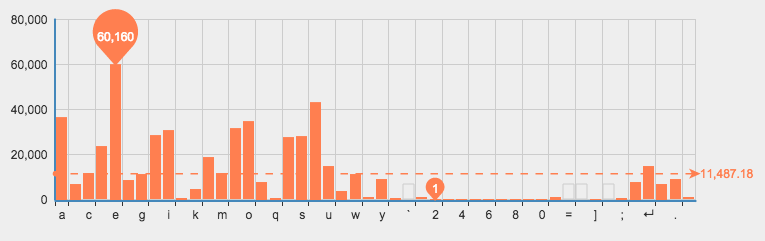
\includegraphics[width=150mm]{img/stats_en}
  \caption{英文资料键位统计图}
  \label{fig:stats_en}
  \end{figure}

  \begin{figure}[h]
  \noindent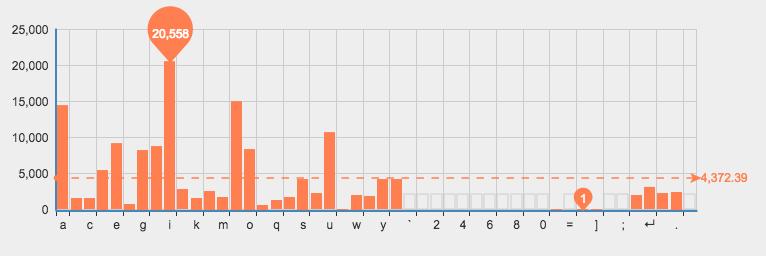
\includegraphics[width=150mm]{img/stats_cn}
  \caption{中文资料键位统计图}
  \label{fig:stats_cn}
  \end{figure}

  \item
  回忆式操作门槛高:拼音输入法要求用户使用之前熟练掌握汉语拼音,不仅如此,还要求用户熟悉每一个汉字的对应拼音组合。结合对键盘布局的考虑,还需要用户熟悉一套键盘设计,了解每一个键的位置。这无疑会增加用户的学习和记忆的负担,对于汉语的初学者来说更是“望洋兴叹”。

  \item
  输入错误修改频繁:用户在使用现有输入法时,往往需要键入声母和韵母之后,浏览过候选汉字,才能意识到自己的输入有误。此时修改输入往往需要连续使用退格键,返回出错位置。这种重复并低效的操作大大影响了用户的输入速度和连续性。

  \item
  声母韵母易混淆:目前所有的拼音输入法均要求用户使用先声母后韵母的输入方式。对某些方言地区的用户来说,分辨声母是很困难的,结合对输入错误修改频繁的讨论,一旦发现输入有误,用户必须删除韵母部分才能修改声母部分。
  \end{enumerate}

  \subsection{现代拼音输入法的新特性\label{sec:new_feature}}

  很多现代拼音输入法做了很多辅助性的工作,意在为用户提供更好地输入体验。

  \begin{enumerate}

  \item
  输入消歧:事实上,拼音作为汉字输入法编码时,重码率非常的高。在GB2312字符集单字重码率上,像五笔、二笔和郑码的重码率都低于5\%,而汉语拼音的编码重码率高达94\%,即使词组重码率上,形码或音形码重码率仍然要比拼音编码重码率低得多。一些研究从结合上下文语义、机器学习等方向对该问题做出了改善。\supercite{wen2008ambiguity, liu2002approach}

  \item
  模糊音:对于不通话不标准的方言地区用户,对常见的易混淆的声母韵母进行了分类。当用户选择开启某一类模糊音选项时,输入法对该选项中的所有易混淆项不加区分。

  \item
  整句输入:随着使用拼音输入法的用户对拼音输入的熟练度逐渐提高,对多字和整句输入的需求明显变高。主流输入法都支持连续输入声母韵母对来输入长句子,不仅增加了输入速度,也能通过上下文语义来消除歧义。

  \item
  生僻字输入:对于不知道读音的生僻字,某一些输入法支持将其从字形上拆解成两个汉字进行输入,只需在输入前加入“u”这个不能作为普通汉字开头的字母即可。如“垚”,输入法下键入“utututu”就可以检索到这个字。
  \end{enumerate}

  \chapter{面向初学者的拼音输入法设计}
  \section{设计初衷}

  对于中国大陆的儿童来说,初级中文教育并不会详细解释如单元音和复元音等等复杂的概念,儿童对韵母构成的理解局限于整体拼写和读音的一一对应关系。而现阶段的拼音输入法都是基于拉丁字母,对尤其是韵母部分,输入时需要进行拆分,如将 “iang” 拆分为 “i”,“a”,“n”,“g” 进行输入。这相当于要求儿童学习拉丁字母以及基于拉丁字母的键盘,对学习拼音输入的儿童来说是一种负担。

  对于国内的一些中老年人,学习中文的时候,并没有掌握学习拼音。对他们来说,复杂的拉丁字母组合也是学习拼音输入一大难题。这一部分用户使用手写输入法为主,会遇到第\ref{sec:current_input}节提到过的问题。尤其考虑到一部分半文盲用户,只具备汉语的听、说、辨识能力,还不具备正确的书写能力,学习拼音输入对他们来说更是难上加难。

  对身居海外的华侨子女,外国人来说,他们学习中文的条件和工具很有限,也是使用的笔画输入法为主。学习使用拼音输入法对他们来说很吃力,将拼音,尤其是韵母拆分为数个拉丁字母进行输入,是一种不直观而且回忆式操作门槛相对较高的方式。特别对有英文输入基础的人,QWERTY键盘反而会有一定程度上的误导性。

  本设计主要面向以上特定人群,⽬的在于克服目前技术中存在的问题,提供⼀种自然的、⾮记忆的中⽂输⼊方法,综合运⽤用汉字多种特征编码,从⽽有效地减少学习负担,提高中⽂输入的效率。当然,对于已经有一定汉语基础,能够熟练掌握汉字声形的用户群体,本设计并不适用。

  此外,考虑到多点触控设备发展迅速,其尺寸有日益增大的趋势,为多点触控等交互手段提供了足够的操作空间。而目前主流拼音输入法中,并没有利用这一优势。本设计希望能充分利用大型触摸设备上多点触控的优势,同时不摒弃原来单点触控的输入方式,提供一种更灵活方便的输入体验。

  \section{设计分析}
  \subsection{布局设计}

  为了达成设计初衷,本设计采用了声母韵母分离,双通道独立输入的方式。基本输入方式与普通输入法相似,即用户通过输入设备输入目标汉字的检索信息,设备根据所属检索信息检索字库,得到候选字集并将所述字集中的汉字按顺序显示于显示屏,用户从所述候选字集选择目标汉字输入。所述检索信息包括声母和韵母两项。

  同时,本设计并没有使用拉丁字母键盘,而是根据拼音的声母和韵母,做出了一套拼音特化的键盘,分为两部分。对于每一个声母和韵母,对应键盘中都会有一个键位与之对应,并在该位置写出拉丁拼写作为标示。声母键盘和韵母键盘分别至多只能有一个键位被按下,其按下的键位的组合代表了用户想要输入的拼音。

  声母韵母的分离设计,有别于现有的QWERTY键盘和手机九键键盘,能使得输入者进行输入时,对声母韵母使用不同手进行操作。根据Kinkead等人的研究\supercite{kinkead},在进行快速打字操作的时候,当手指的操作速度达到理论最值,那么键盘布局对输入速度的影响非常之小。然而,基于人类手掌的结构,一般来说,同一只手的连续操作速度会比两只手间断操作稍慢。因此,本设计将按键顺序严格限制为左右手间隔操作,意在提高用户的输入速度,与德沃夏克键盘布局将元音辅音尽量做两极化的思想类似。

  \subsection{交互设计}

  一般拼音输入法要求用户以首先输入声母,再输入韵母的方法进行输入。虽然现代拼音输入法在词组匹配,长句输入,自动纠错上做了很多贡献,但这种顺序输入的方式依然没有改变。如果在输入长句子时键入了错误的声母,就意味着需要删除到错误的点进行重新输入。由于韵母数量多于声母,如果存在有独立的两个检索通道,不要求先后的顺序关系,尤其对初学者来说,会有更多选择的余地。

  本设计考虑到了初学者的这一需求,没有强制声母和韵母的输入顺序,用户可以任意顺序输入声母和韵母,亦可在支持多点触控的平板上,同时输入声母韵母。

  考虑到声母韵母之间的搭配并非任意,而是存在一定的规则。例如,声母 “p” 与韵母 “iong” 、声母 “n” 与韵母 “ia” 等等,没有任何汉字与其读音相匹配。考虑到这种规则并没有一个清晰且容易记忆的规律,对初学者用户来说,这也是学习拼音输入的一大难点。本设计做了对初学者友好的提示设计,当声母和韵母其中一个被选中时,另一个输入区只会显示能够匹配上至少一个汉字的键位,并隐藏其他键位。例如,当韵母 “v” 被选中时,声母区只有 “l” 和 “n” 显示给用户,而其他键位都隐藏。当声母和韵母同时被选择时,则显示所有的声母和韵母键位。

  \section{具体实现}
  \subsection{整体布局}

  输入法的整体布局如图\ref{fig:layout1_background}所示。整个布局分为上下两部分。上部分为汉字显示区,会依次显示用户所输入的汉字。输入区右下角浅色的方框为拼音显示区,用于提示用户当前激活的声母以及韵母。下部分又细分为左、中、右三个子部分。左右两个子部分,分别是声母和韵母输入区,中间区域是汉字备选区。

  \begin{figure}[h]
  \noindent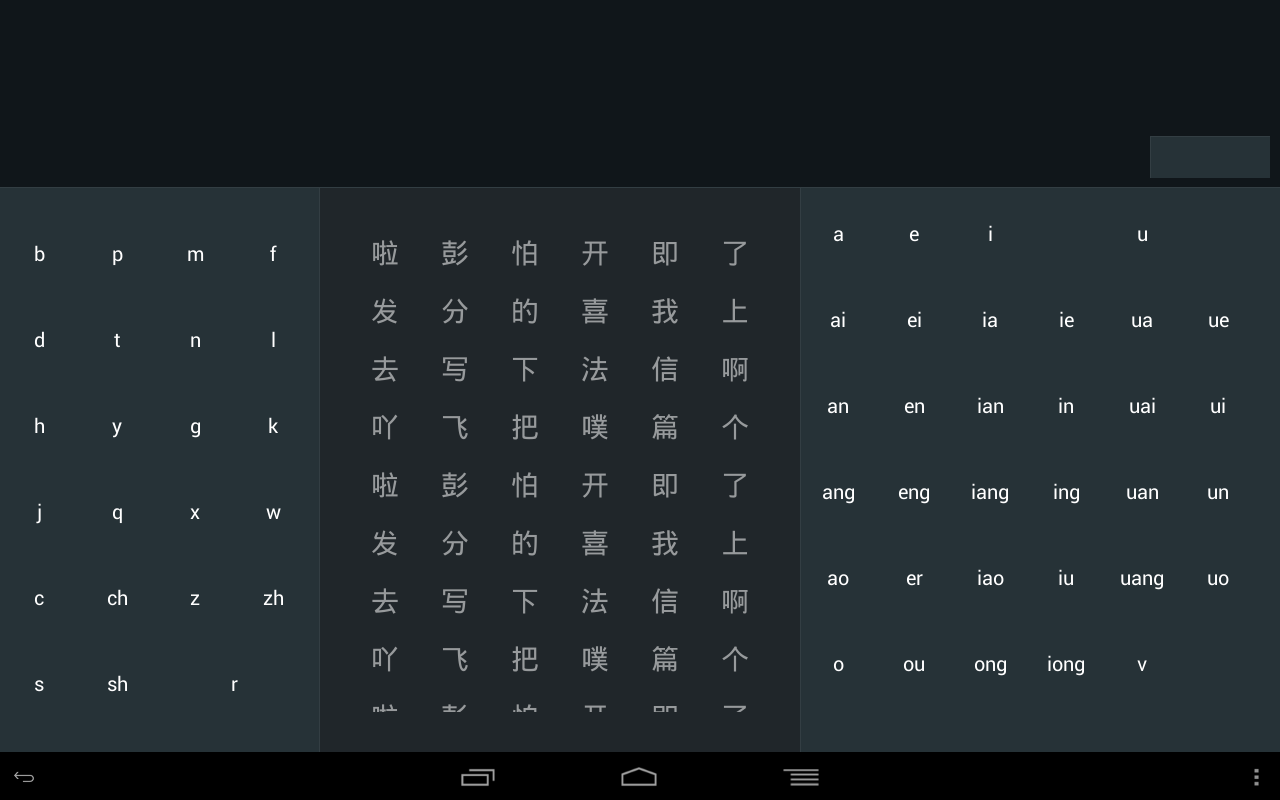
\includegraphics[width=150mm]{img/layout1_background}
  \caption{输入界面}
  \label{fig:layout1_background}
  \end{figure}

  可以看到,声母区和韵母区没有依照拉丁字母构建,完全是自定义键盘,键位涵盖了所有声母和韵母。中间部分采用大面积候选表格代替了传统的候选行,使用户能够看到更多的候选汉字。

  \subsection{输入区布局设计}

  声母输入区的键位采用了“发音部位-发音方法”的排列方法。如 ”b“、”p“ 均为双唇音,区别在于 ”b“ 是不送气音,”p“是送气音。因此,在键盘排布上,将 ”b“、”p“ 放在一行。依照“发音部位-发音方法”,将声母排列成为六行四列的表格。这种组合有两个优势:其一,使用距离远近加工了声母的近似程度,能够在初学者用户输入时给予暗示,加速其学习的速度;其二,对于不同地区的方言对声母的不区分现象主要发生在近似程度较高的声母间,输入法可以将相邻声母键位融合成一个来达到模糊输入的效果。关于对方言地区用户的输入优化在第\ref{sec:dialect}节有详细介绍。

  韵母输入区的布局思路类似声母输入区,采用”口型-元音类型“进行分类。其目的和优势都是相同的。

  声母输入区和韵母输入区均采用了无边框键位设计。根据Chaudhri等人的论述\supercite{chaudhri},目前多数虚拟键盘设计沿袭了物理键盘,采用了仿真式的视觉设计。然而,在触摸屏幕上操作,并没有实体键盘的触觉反馈,事实上只有位置信息这一个输入。这样的视觉设计是无法有效的避免误操作的。因此,本设计在视觉效果上,参考google拼音输入法\footnote{\url{https://play.google.com/store/apps/details?id=com.google.android.inputmethod.pinyin&hl=en}}采用了无边框设计。无边框设计虽然依旧无法对误操作进行改善,但能够使得整个界面看起来简单,布局明朗。

  \subsection{输入区交互设计}

  本实现包括一种过滤模块。该模块会被用户触摸屏幕事件所激活,接受并保存触摸的位置信息,并且将触摸位置映射为用户动作。具体来说,如果触摸事件位置在由于声母输入区、韵母输入区和汉字备选区,则认为此次操作是一次有效的输入操作,根据触摸位置,判断用户所希望按下的键位。其他区域的触摸事件被当做无效操作,从而忽略。对于多点触摸设备,一个输入区的多个触摸事件会产生输入冲突。在这种情况下,判断其为无效操作。而对于不支持多点触摸的设备,则不会产生冲突。

  与设计的初衷一致,当声母输入区有一个键位按下时(韵母区尚未操作),韵母区所有不能与该声母匹配的键位暂时消失,以提示用户。(见图\ref{fig:layout1_s_press_down})此时,如果用户在余下的韵母中选择了一个键位,则重新显示所有韵母输入区内容,并且在汉字备选区中加入满足该组合的所有汉字,按照使用频率降序排列。类似的,当韵母按下时,无法匹配的声母也会暂时消失。

  \begin{figure}[h]
  \noindent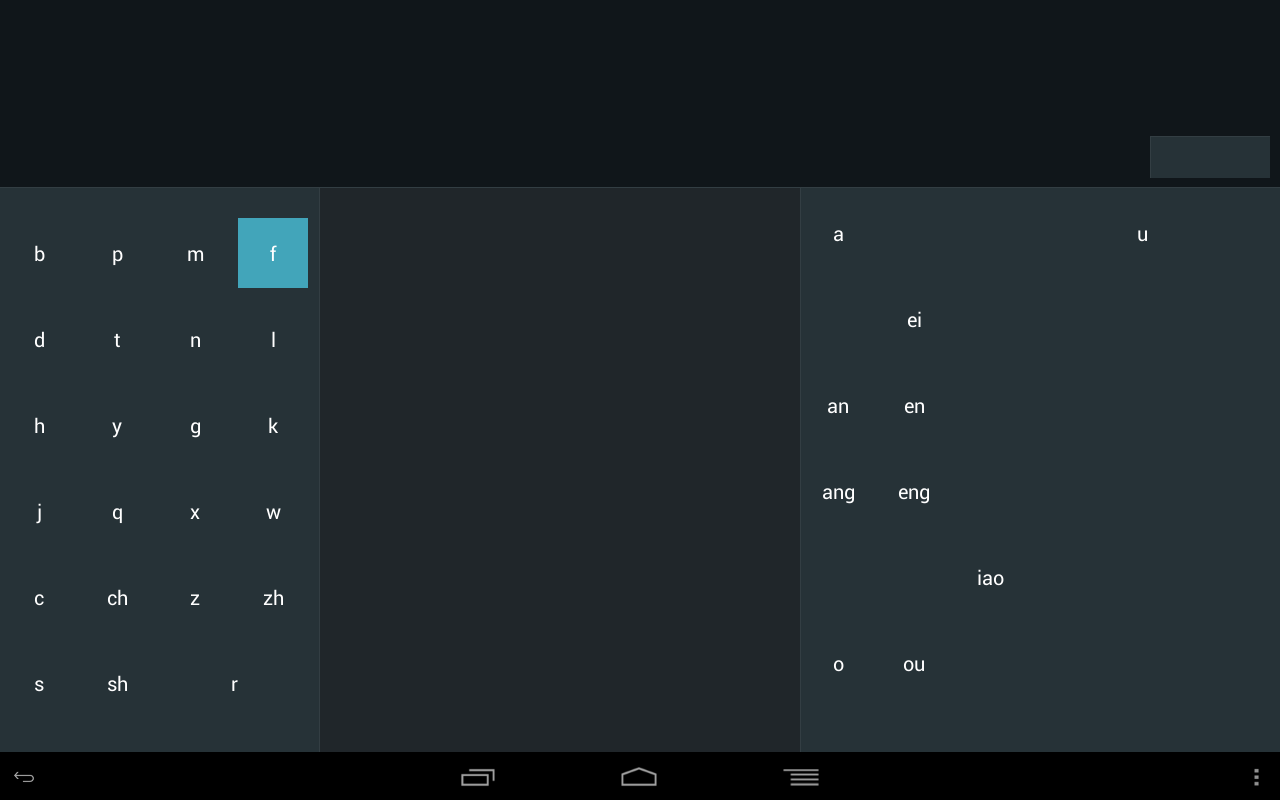
\includegraphics[width=150mm]{img/layout1_s_press_down}
  \caption{声母键位按下}
  \label{fig:layout1_s_press_down}
  \end{figure}

  当声母和韵母都有正确输入时,符合其音律组合的汉字会出现在汉字备选区中。汉字备选区采用了六列若干行的表格的形式,支持两种不同的操作:点击某一个汉字键位,表示用户选择了这一个汉字,该汉字会出现在上部汉字显示区中,并在拼音显示区显示当前输入的声母韵母组合(见图\ref{fig:layout1_finished});垂直拖动汉字备选区,表示用户希望选择的汉字没有出现在表格中,表格将上下滚动以显示更多内容。备选区选择表格这种形式,也是考虑到初学者对汉字不熟悉的情况,给予其更多汉字选择。

 % \begin{figure}[h]
 % \noindent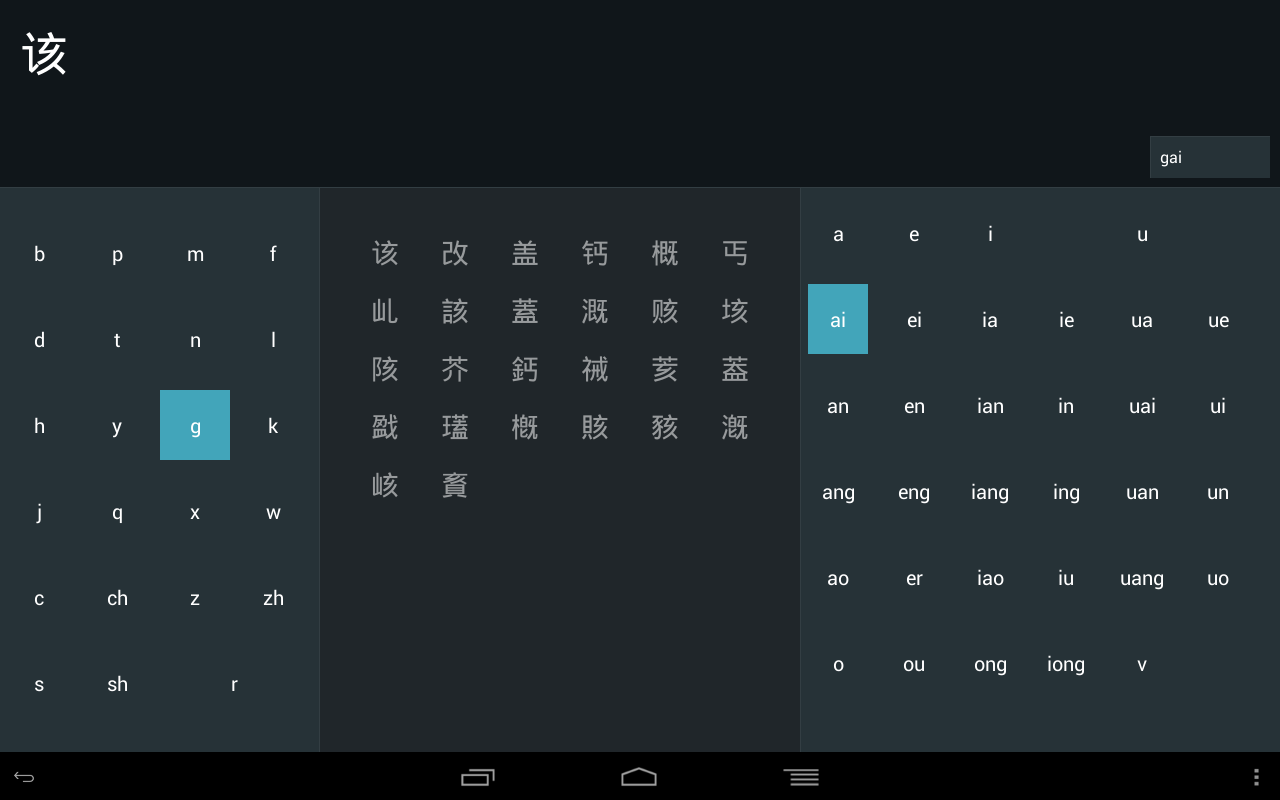
\includegraphics[width=150mm]{img/layout1_finished}
 % \caption{选择汉字操作}
 % \label{fig:layout1_finished}
 % \end{figure}

  \section{本设计的优势}

  通过与现有拼音输入法进行对比,充分考虑到第\ref{sec:limit}节所提到的现有输入法的局限性,本设计的优势有以下几点:

  \begin{enumerate}
  \item
  依托多点触摸技术,实现⾃然⽅式交互:由于该设计采用了多点触控的技术,赋予了用户更多操作的空间。例如:用户在实际操作中可以使用一个手指输入声母后保持不变,另一个手指输入韵母,双手并用,而无需像在单点触摸屏,点击后马上抬起。双⼿并用、多指操作这是最自然、最舒适的输⼊方式,符合⼤多数⼈的操作习惯,而这种自然的交互⽅式也势必是人机交互未来发展的⽅向。

  \item
  拓展多通道技术,提出韵母检索新⽅式:多通道(multi-modal,也称多模式)交互模式已被诸多研究证明是提高交互效率和自然性的有效途径。多通道交互作为未来人机交互中的一项核心技术在国内外受到了普遍的关注。\supercite{dsh,lmz}用户可以通过各种不同的交互通道以及它们之间的相互组合、协作来完成交互任务,这正好弥补了单一交互模式给用户带来的限制和负担。本设计中涉及的拼⾳声母和拼⾳韵母都以独立的显示区域存在,并且以其中任何一个作为输⼊时都可以表达⽤户的输⼊意愿,其输入内容互不相关、输出结果相互补充,在操作时具有前后⽆关性,更改其中一个的输⼊即可实现结果的修正,因此我们可以将其看作是两个独立的输⼊通道。由于拼⾳韵母是一个独⽴的输⼊通道,我们可以实现韵母的检索和提示模式,能够回避⽤户对声母混淆的问题,有效降低输入时的出错率。对于⽬前主流的单点触摸设备,本设计仍然适用。声母表区和韵母表区可以记录并保存⽤户的最后一次输入,用户可以任意顺序依次在两个区域完成输入。

  \item
  人性化设计输入界⾯面,学习记忆⽆无负担:输入界面的设计采用人体工效学的方法科学设计,具体表现为:布局合理,声母区和韵母区分别使用“发音部位-发音方法”和“口型-元音类型”的原则排列,易于用户记忆和熟练操作后提高输入速度。另外,本设计已将所有的声母、韵母以及组合完整的显示出来,用户所需的操作仅是从屏幕中罗列的拼⾳中选择⾃己认为正确组合情况,避开了繁重和易于混淆的记忆过程。

  \item
  ⽤户群体广泛,与现有输⼊法形成互补:与设计初衷一致,本设计大量考虑了拼音输入的初学者,包括学龄儿童、老人、半文盲、外国华侨及其子女等等人群,充分考量他们对学习拼音输入的困难,并从各个方面为其定制功能和外观。本发明合理的弥补了传统汉字输入法流失的⽤户群体,并与其组成了一套完整的汉字输⼊体系,能够满足所有有意愿学习和应⽤用汉语的人的要求,这势必会对汉语的普及和教育起到极大的推动作用。
  \end{enumerate}

  \chapter{面向熟练者的拼音输入法设计}
  \section{设计初衷}

  大多数18到30岁左右用户都受过良好的教育,拼音基础知识牢固,已经有十年以上的拼音输入法使用经验,并且能够熟练地使用除基础输入以外更多新增特性。(见第\ref{sec:new_feature}节)在上一章的讨论中,我们把这一部分用户列为非初学者用户,不妨称其为熟练者。由于熟练者对拼音掌握的程度远远高于初学者,我们可以假定,他们在拼音形态的辨识,拼音与汉字的匹配方面不存在任何困难。因此他们在触摸设备上的输入体验更多的局限于现有键盘的布局和交互技术。

  正如之前第\ref{sec:limit}节所讨论的一样,现有拼音输入法键盘,无论是QWERTY键盘还是九键键盘,并不是为拼音输入定制的。再者现有的拼音输入法大多采用点击输入的方式。无论单点触摸设备还是多点触摸设备,其基本的交互方式都是在屏幕同一位置按下和抬起,手指离开屏幕后才会有位移动作。事实上,触摸设备提供了更加丰富的交互体验,例如单指滑动,双指收缩等等,输入法程序并没有很好地利用起来。

  本设计主要面向熟练的拼音输入用户,目的在于克服传统键盘所带来的输入局限性,根据韵母自身的特性进行拆分,提供一种充分利用大型多点触摸设备所提供的交互功能,布局更紧凑的中文输入方法,提高中文输入效率和体验。

  \section{设计分析}
  \subsection{布局设计}

  基本的布局设计思路与面向初学者的设计类似。考虑到汉语拼音的多元音韵母形式上是由单元音韵母拼合而成,熟练者已经掌握所有多元音韵母的组成,我们考虑在韵母输入区只保留单元音韵母,单元音韵母使用简单的触摸动作输入,多元音韵母则使用滑动输入。

  \subsection{交互设计}

  一些可视化研究在触摸屏幕上使用了很多丰富的交互,包括一些图表上操作技术\supercite{sadana2014designing},通过显示用户输入位置热图来纠正用户操作\supercite{rudchenko2011text},。有些研究甚至考虑到了触摸设备两面的可操作性,来延伸交互的可能\supercite{buschek2014improving, shen2009double}。一些在输入法也在交互手段上做了创新,包括一些基于QWERTY键盘的变体\supercite{findlater2012beyond, shin2009multi},将键盘分离为负责区域和负责细节两个部分分别输入\supercite{don2010applying},移出某些容易造成误操作的键位\supercite{arif2014experimental}等等。这些思路都在某种程度上说明在输入法用户界面使用更丰富的交互手段是可行的并且是有效的。

  事实上,在英文的虚拟键盘上,轨迹输入早已出现\supercite{kristenssondiscrete, hinckley2002input, zhai2008interlaced},主要思路比较相似,都是储存用户输入轨迹,与标准轨迹计算相似程度,其中计算相似程度的算法多样。本设计沿袭了这一过程,使用了比较简单直接的相似度算法,应用在自定义的韵母输入区键盘上。

  \section{具体实现}
  \subsection{输入区布局设计}

  输入法的整体布局如图\ref{fig:layout2_background}所示。与面向初学者的布局类似,不再赘述。

  \begin{figure}[h]
  \noindent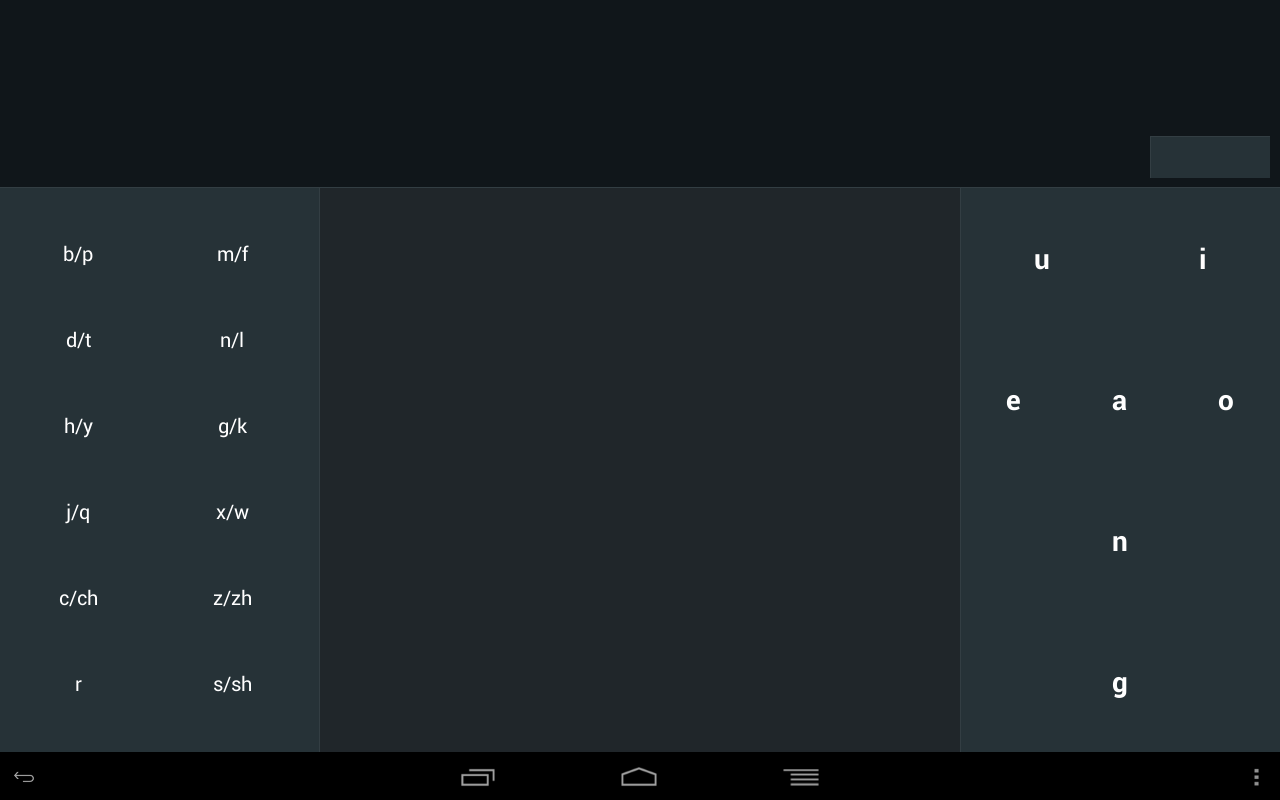
\includegraphics[width=150mm]{img/layout2_background}
  \caption{输入界面}
  \label{fig:layout2_background}
  \end{figure}

  可以看到,声母区的相邻声母进行了合并,这是为了第\ref{sec:dialect}节所做的实验性步骤,在改节有详细说明。韵母区只保留了单元音韵母,并对其排列进行了调整,使得所有其他多元音韵母都能够通过单元音组合而成,并使得其轨迹比较平滑规整。

  \subsection{输入区交互设计}

  由于声母的特殊性,无法向韵母一样拆分,故声母区的输入方式与面向初学者的没有区别。同样的,汉字备选区,汉字显示区和拼音提示区都与之前设计无差别,因此不再赘述。

  韵母区的操作分为两种:

  \begin{enumerate}
  \item
  点击:对于单元音韵母的输入,与之前的设计没有区别,直接点击对应键位即可。

  \item
  滑动:对于多元音韵母的输入,需要用户使用“滑动”这一交互手段。所谓滑动,即是在某一位置接触屏幕,保持接触并在同时移动手指,到另一位置放开手指。例如要输入 “iang” ,就需要在键位 “i” 按下,拖动手指经过 “a”,“n” 直到到达 “g”,然后放开手指。用户手指轨迹以及检索结果见图\ref{fig:layout2_input}

  \begin{figure}[h]
  \noindent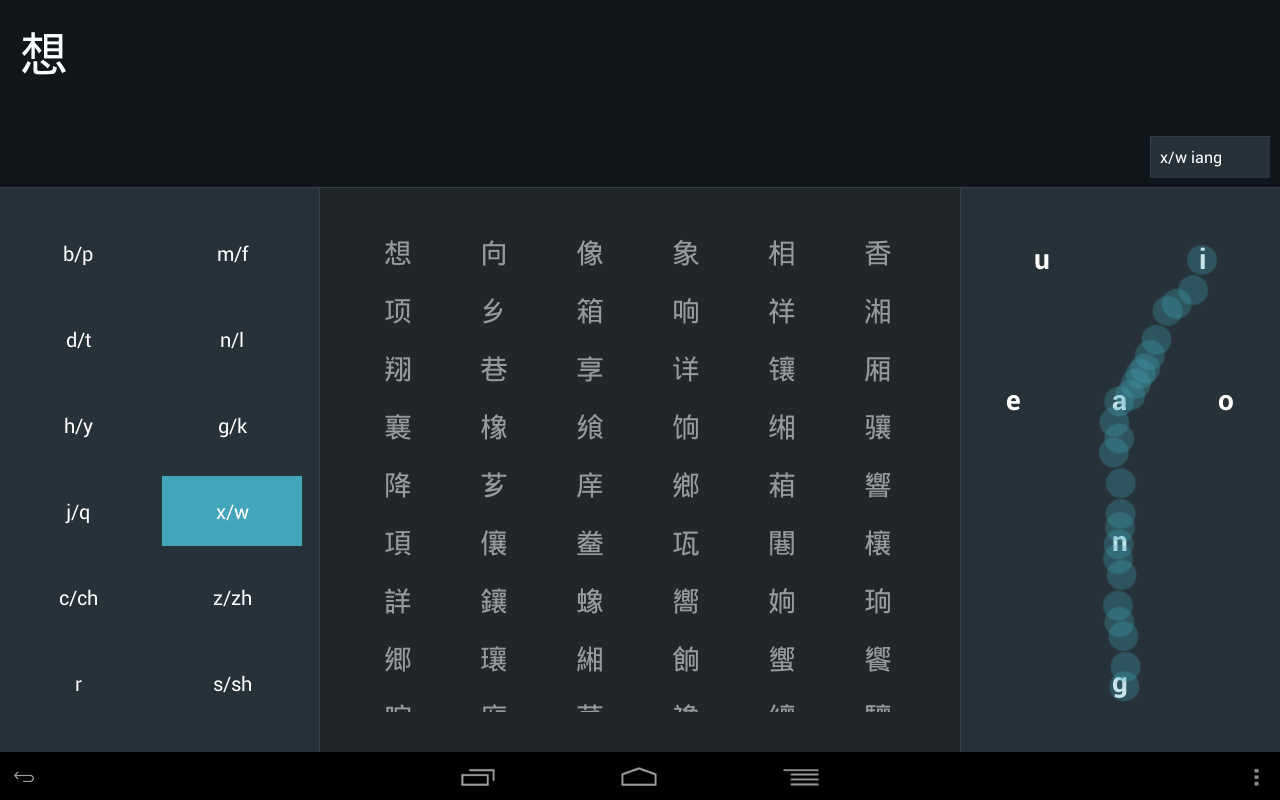
\includegraphics[width=150mm]{img/layout2_input}
  \caption{滑动输入}
  \label{fig:layout2_input}
  \end{figure}

  \end{enumerate}

  \subsection{轨迹相似度算法\label{sec:tra_algorithm}}

  本实现使用了最简单最直接的相似度算法。假设有二维平面点\(v = (x, y)\)。定义每一个单元音韵母有唯一坐标,为键位中点,得单元音韵母坐标集\(S = \{v_0, v_1, \dots, v_6\}\)。定义多元音韵母标准轨迹为其每个元音对应韵母的坐标依次连接所得的折线,即\(s = (v_{i_1}, v_{i_2}, \dots, v_{i_n}), (n \leq 6)\),其中\(I = \{i_1, i_2, \dots, i_n\}, (n \leq 6) \)为某一多元音韵母拆分成的单元音韵母在单元音韵母坐标集合中的下标。定义标准轨迹集\(S = \{s_0, s_1, \dots, s_n\}\)。

  此时,用户的滑动输入可以看做是一组点集,记为\(W\), 记点到直线距离函数为\(disL(v_1, v_2, v_3)\),表示点\(v_1\)到\((v_2, v_3)\)所在直线的欧式距离。在定义点到标准轨迹的距离:

  \[disS(v', s) = \min_{v_i \in s }\{disL(v', v_i, v_{i+1})\}\]

  由此我们定义相似度为

  \[q_i = \frac{1}{\sum_{v \in W}\,disS(v, s_i)}, (s_i \in S)\]

  相似度越大,我们认为轨迹\(W\)与标准轨迹\(s_i\)在位置上越相似,用户更倾向于选择标准轨迹为\(s_i\)的韵母。相似度最大为正无穷,即用户轨迹精准的落在标准轨迹上。

  最后,在所有相似度中求得最大的一项\(\max(q_0, q_i, \dots, q_m)\)所对应的韵母即视为用户的输入。

  算法的具体代码详见附录\ref{sec:code}。

  \subsection{本设计的优势}

  同样,考虑第\ref{sec:limit}节所提到的现有输入法的局限性,本设计的优势包括前一设计的1、2、3点以外,还有以下几点:

  \begin{enumerate}
  \item
  缩减键盘空间,使盲打成为可能:由于本设计的韵母键盘压缩了相当大的空间,使得用户可以在大型触摸设备上,双手握住设备边缘,仅靠左右手大拇指即可操作。虽然以目前的设计来看,选择汉字还是需要更多手指配合,但这已经是一大进步了。再者,由于单元音数量较少,熟练者在掌握本输入法后,在右手实现盲打的可能性较高。

  \item
  丰富交互方式,充分利用设备:在自定义韵母输入区键盘上,使用了滑动输入的方式,改进目前输入法单一的触摸交互方式。这一改善不仅充分利用了触摸设备提供的交互功能接口,还为输入法用户提供了一次新鲜的交互体验。相信随着更加完善的研究和成熟的发展,更丰富的交互手段一定会踏上输入法这一块土地。

  \end{enumerate}

  \chapter{比较与拓展}

pkuthss~文档模板的源代码中已经有了较为详细的注释,
故请直接参照相应文件中的注释。

\emph
{%
	注:%
	img~目录中的~Makefiles~和两个~PostScript(\texttt{.ps})%
	文件中也有详细的注释哦~:)
}


  % 结论。
  \specialchap{结论}

本文在介绍了现有拼音输入法,通过调研分析了现有输入法对某一些用户的不适用性,通过辅助性程序分析了现有拼音输入法键盘的非最优性。之后,本文将现有主要拼音输入法用户根据对汉语拼音及拼音输入法的熟悉程度分为两类,详细讨论了两种不同用户群对中文拼音输入法的需求差异,分析了现有输入法对于不同用户群的不同劣势。

针对两组用户的需求差异,本文分别做出了面向这两种用户的输入法设计,研讨了设计初衷,提出了设计方案,并初步在Android设备上实现了设计。对于初学者用户群体,采用了全声母韵母分离式键盘设计,结合多通道、多点触控技术,为其创造了一个记忆负担小,上手快,有一定辅助学习功能的输入环境。对于熟练者用户群体,采用了全声母键盘,辅以精简韵母键盘,在前者的基础上,充分利用了现代多点触控设备提供的滑动交互功能,为用户提供了一种新型的,交互形式丰富,占用空间少,有一定盲打可能性的输入环境。

当然,设计本身和初步的实现都还有很多不足的地方。本文提出了一些目前实现的不足之处,对其后续发展提出了相应的讨论。如对整句输入的支持,布局的改进以及算法的优化等等。除此之外,我相信在多点触摸设备上,尤其是大型设备上的拼音输入法还有更多的地方值得探索和挖掘。


  \begin{appendix}
    % 参考文献。
    \bibliographystyle{chinesebst}\bibliography{sample}
    % 此命令手动地在目录中增加相当于章级别的一行。
    \addcontentsline{toc}{chapter}{\bibname}
    % 此命令和真实的一级章命令结合,从而使 \addcontentsline
    % 在目录中产生的页码正常。
    \phantomsection

    % 各附录。
    \chapter{代码统计}

主程序代码是两种输入法在Android系统上的实现。包括两种布局的实现,各种按键交互的时间,轨迹算法的实现等等。\footnote{代码统计使用工具cloc: \url{http://cloc.sourceforge.net/},下同}

\begin{table}[h]
  \begin{tabular*}{150mm}{@{\extracolsep{\fill} } l || r || r || r || r }
  \hline
  语言 & 文件数 & 空行数 & 注释 & 实际代码量 \\
  \hline
  Java & 13 & 310 & 602 & 2463 \\
  XML & 26 & 117 & 14 & 1582 \\
  \hline
  SUM: & 39 & 427 & 616 & 4045 \\
  \hline
  \end{tabular*}
  \caption{主程序代码量统计}
  \label{table:main_stats}
\end{table}

辅助小程序是用于统计txt文本中拉丁字母和中文汉字所使用的QWERTY键位的次数,并画出热图及统计图。(见第\ref{sec:limit}节)程序以交互式网页的形式呈现,在\url{http://hacker-yhj.github.io/projects/keyboardStroke/index.html}可以访问。

\begin{table}[h]
  \begin{tabular*}{150mm}{@{\extracolsep{\fill} } l || r || r || r || r }
  \hline
  语言 & 文件数 & 空行数 & 注释 & 实际代码量 \\
  \hline
  HTML & 1 & 38 & 6 & 393 \\
  Javascript & 1 & 9 & 0 & 161 \\
  \hline
  SUM: & 2 & 47 & 6 & 554 \\
  \hline
  \end{tabular*}
  \caption{辅助程序代码量统计}
  \label{table:aux_stats}
\end{table}

  \end{appendix}

  %% 以下为正文之后的部分,页码为大写罗马数字。
  \backmatter\pagenumbering{Roman}

  % 致谢。
  \chapter{致谢}

在学士学位论文即将完成之际,我想向曾经给我帮助和支持的人们表示衷心的感谢。首先要感谢我的导师王衡教授,她在学习和科研方面给了我大量的指导,并为我们提供了良好的科研环境,让我学到了知识,掌握了科研的方法,也获得了实践锻炼的机会。她严谨的治学态度、对我的严格要求使我受益匪浅。除此之外,她在《人机交互》课程上毫无保留的解答了我对未来发展方向的解惑,也让我受用终身。在此向她表示由衷的感谢!

感谢我已经毕业的师兄邓德重、邓景文,师姐化静,他们曾经给了我无私的帮助和鼓励,让我学到很多。感谢实验室同僚钱锦,王文铎,他们丰富的经验和科研的热情对我的论文设计提供了很大的支持。感谢同届的徐鹏,师弟吕鑫,江天源,他们是我学习、工作和生活上的伙伴,也是面对困难和挑战时的战友。和他们在一起的日子是本科期间快乐的时光。

感谢我在可视化实验室实习时,我的导师袁晓如对我的悉心教导。他在我对科研一无所知的时候,让我参与内部组会,熟悉计算机科学研究,尤其是可视化方向研究的流程,让我领略了科研的严谨冷峻的魅力。虽然我最后没有在可视化实验室一直实习下去,但他对我的投入,与我之后的实习的选择以及未来方向的选择,都是分不开的。

感谢在北京微软亚洲研究院实习时的同事们,他们在我第一次参加实际项目开发的过程中给了我莫大的帮助和鼓励。特别要感谢我的项目经理张海东,我的mentor Ray,胡志涛,是他们的信任给了我很多锻炼的机会,也一直对他们给予我的生活上的照顾心存感激。和他们一起为可视化项目奋战的一年多是我人生中一段难忘的经历。

感谢我在创业公司的同事们,董未、向仁凯、张哲、王杨,他们的精湛专业技能和严谨的做事风格永远是我学习的榜样。更多我无法逐一列出名字的朋友,他们给了我无数的关心和鼓励,也让我的本科校外生活充满了温暖和欢乐。我非常珍视和他们的友谊!

感谢信息科学技术学院计算机系3班的同学,感谢他们在学习和生活上给予我的帮助。

感谢我的父母,他们给了我无私的爱,我深知他们为我求学所付出的巨大牺牲和努力,而我至今仍无以为报。祝福他们,以及那些给予我关爱的长辈!

还有很多我无法一一列举姓名的师长和友人给了我指导和帮助,在此衷心的表示感谢!

最后,衷心感谢在百忙之中抽出时间审阅本论文的专家教授。

  % 原创性声明和使用授权说明,不显示页码。
  \cleardoublepage\pagestyle{empty}
  \cleardoublepage
\section*{北京大学学位论文原创性声明和使用授权说明}
\vfill

\section*{原创性声明}

本人郑重声明:
所呈交的学位论文,是本人在导师的指导下,独立进行研究工作所取得的成果。
除文中已经注明引用的内容外,
本论文不含任何其他个人或集体已经发表或撰写过的作品或成果。
对本文的研究做出重要贡献的个人和集体,均已在文中以明确方式标明。
本声明的法律结果由本人承担。
\vspace{2.5em}\par

\rightline
{%
	论文作者签名:\hspace{5em}%
	日期:\hspace{2em}年\hspace{2em}月\hspace{2em}日%
}
\vfill

\section*{学位论文使用授权说明}
\vspace{-1em}\par
\centerline{\zihao{-4}(必须装订在提交学校图书馆的印刷本)}
\vspace{1em}\par

本人完全了解北京大学关于收集、保存、使用学位论文的规定,即:
\begin{itemize}\denselist
	\item 按照学校要求提交学位论文的印刷本和电子版本;
	\item 学校有权保存学位论文的印刷本和电子版,
		并提供目录检索与阅览服务,在校园网上提供服务;
	\item 学校可以采用影印、缩印、数字化或其它复制手段保存论文;
	\item 因某种特殊原因需要延迟发布学位论文电子版,
		授权学校~\Square~一年~/\Square~两年~/\\
		\Square~三年以后在校园网上全文发布。
\end{itemize}
\par(保密论文在解密后遵守此规定)
\vspace{2.5em}\par

\rightline
{%
	论文作者签名:\hspace{5em}导师签名:\hspace{5em}%
	日期:\hspace{2em}年\hspace{2em}月\hspace{2em}日%
}


\end{document}

